\subsection{Otras reprenseaciones del problema}
Durante el desarrollo de este trabajo se han probado diferentes representaciones
del problema, con el objetivo de buscar la que mejor se adapte al modelo. En
esta sección se van a explicar las diferentes representaciones que se han probado
y se va a justificar la elección de la representación final.\medskip

\subsubsection{Representación con construcción secuencial}
\begin{itemize}
    \item Espacio de estados: El estado puede ser representado por una 
    lista de máquinas, donde cada máquina tiene una lista de operaciones asignadas
    a ella. Puede utilizar una estructura de datos como una matriz o una lista de
    listas para representar este estado. Cada elemento de la lista puede contener 
    información sobre la operación, como su duración, prioridad u otras características 
    relevantes.
    \item Espacio de acciones: Las acciones posibles consisten en asignar una operación 
    a una máquina específica o realizar un cambio de máquina. Es posible representar las acciones 
    mediante un conjunto de códigos que identifiquen cada acción. Por ejemplo, puedes asignar 
    un número a cada máquina y utilizar números adicionales para representar acciones 
    de cambio de máquina.
    \item Transiciones de estado: Cuando el agente asigna una operación a una máquina, 
    el estado se actualiza con la nueva asignación. Si el agente decide cambiar de máquina, 
    el estado se actualiza para reflejar la nueva máquina activa y las operaciones restantes.
\end{itemize}
\subsubsection{Representación mediante imagen con eliminación}
\begin{itemize}
    \item \textbf{Espacio de estados:} El estado se representa por una imagen que contiene 
    los posibles tiempos de finalización de las operaciones. Existe una matriz de píxeles 
    para representar la imagen, donde cada píxel representa el tiempo asociado a una operación 
    en una posición específica. Por ejemplo, el valor de un píxel podría representar el tiempo 
    de finalización estimado de una operación en una determinada ubicación.
    \item \textbf{Espacio de acciones:} Las acciones posibles consisten en eliminar zonas de 
    la imagen. Puedes representar las acciones mediante coordenadas que delimitan un área a 
    eliminar en la imagen. Por ejemplo, una acción podría estar representada por las 
    coordenadas de dos esquinas de un rectángulo que define la zona a eliminar.
    \item \textbf{Transiciones de estado:} En este caso, cuando el agente elimina una zona de 
    la imagen, el estado se actualiza reflejando la nueva configuración de tiempos de finalización. 
\end{itemize}
\subsubsection{Representación con grafos y nodo de cambio de máquina}
\begin{itemize}
    \item \textbf{Espacio de estados:} Cada estado se representa por un grafo 
    que representa la configuración actual de una máquina. Cada nodo del grafo puede representar 
    una operación, y las aristas representar las dependencias entre ellas. Se le asignan
    características a los nodos, como el tiempo de procesamiento de la operación o cualquier 
    otra información relevante.
    \item \textbf{Espacio de acciones:} Las acciones posibles pueden ser cambiar de máquina 
    o realizar una operación en la máquina actual. Puedes representar las acciones mediante 
    un código que identifique cada operacion y la maquina en la que se va a asignar. Por 
    ejemplo, una acción puede estar representada por un código que indique cambiar de máquina o 
    un código que indique realizar una operación específica en la máquina actual.
    \item \textbf{Transicion de estado:} Las transiciones de estado ocurren cuando el agente 
    toma una acción y el entorno se actualiza en consecuencia. Cuando se realiza una operación 
    en la máquina actual, el grafo de la máquina se actualiza para reflejar el cambio de estado. 
    Si se decide cambiar de máquina, se puede utilizar un nodo especial en el grafo para representar 
    la transición a otra máquina.
\end{itemize}
\begin{figure}[ht]
    \centering
    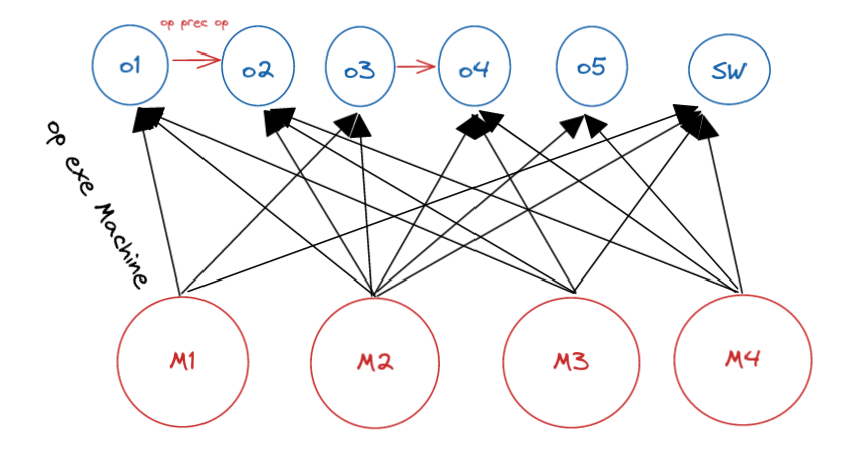
\includegraphics[scale=0.4]{graphv0.png}
    \caption{Representación mediante grafos con nodo de cambio de máquina}
    \label{fig:rep-graph-v0}
\end{figure}
